\documentclass{standalone}
%\pagenumbering{gobble}


%%%%%%%%%%%%%%%%%%%%%%%%%%%%%%%%%%%%%%%%%%%%
% shock schematic
%
%%%%%%%%%%%%%%%%%%%%%%%%%%%%%%%%%%%%%%%%%%%%


\usepackage{tikz,xcolor}
\usetikzlibrary{arrows, shadings, calc}

\begin{document}

\tikzset{
	level/.style={thick},
	trans/.style={thick, dashed,->,shorten >=2pt,shorten <=2pt,>=stealth},
	photon/.style={thick, ->, snake=snake, line after snake=1mm}
	}


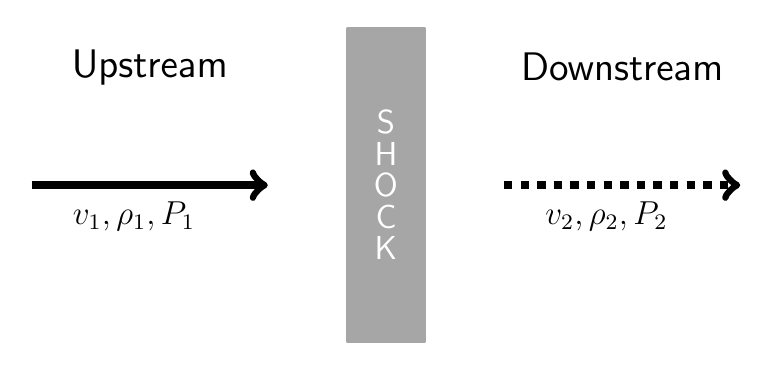
\begin{tikzpicture}[scale=1.0, font=\sffamily]

	\node[align=center] at (1.5,1.5) {\Large Upstream};
	\draw[thick, line width=1mm, ->] (0,0) -- (3,0);
	\node[align=center] at (1.3,-0.4) {\large $v_1, \rho_1, P_1$};

	\node[align=center] at (7.5,1.5) {\Large Downstream};
	\draw[thick, line width=1mm, dashed, ->] (6,0) -- (9,0);
	\node[align=center] at (7.3,-0.4) {\large $v_2, \rho_2, P_2$};

	% shaded area for shock
	\begin{scope}%[transform canvas={rotate=30}]
		%\shade[shading=axis,bottom color=black,top color=white, shading angle=-90] (4,-2) rectangle (5.5,2);
		\shade[shading=axis,bottom color=gray!70,top color=gray!70, shading angle=-90] (4,-2) rectangle (5.0,2);
	\end{scope}
	\node[align=center, white] at (4.5,0.8) {\large S};
	\node[align=center, white] at (4.5,0.4) {\large H};
	\node[align=center, white] at (4.5,0) {\large O};
	\node[align=center, white] at (4.5,-0.4) {\large C};
	\node[align=center, white] at (4.5,-0.8) {\large K};

\end{tikzpicture}

\end{document} 
